%\documentclass[12pt,a4paper]{article}
%
%\usepackage{amsmath, amssymb}
%\usepackage[utf8]{inputenc}
%\usepackage[english]{babel}
%\usepackage{graphicx}
%\usepackage[margin=0.5in]{geometry}
%\usepackage{float}
%
%\graphicspath{{fig/}}
%
%
%\begin{document}

\subsection*{Level 2}
The velocity controller from Exercise 3 was used as controller. Following the first part of the task the chosen values can be seen in the following table.

\begin{center}

	\begin{tabular}{| c | c |}
		\hline
		Am & 500 \\ \hline
		$Ao_1$ & 1000 \\ \hline
		$Ao_2$ & 2000 \\
		\hline
		

	\end{tabular}

\end{center}

\subsection{}
Figure \ref{fig:task3_1_1000} shows the step responses for two different values of Ao. A force of 5000 N is applied at the time 0.03 seconds.
\begin{figure}[H]
	\begin{center}
	
		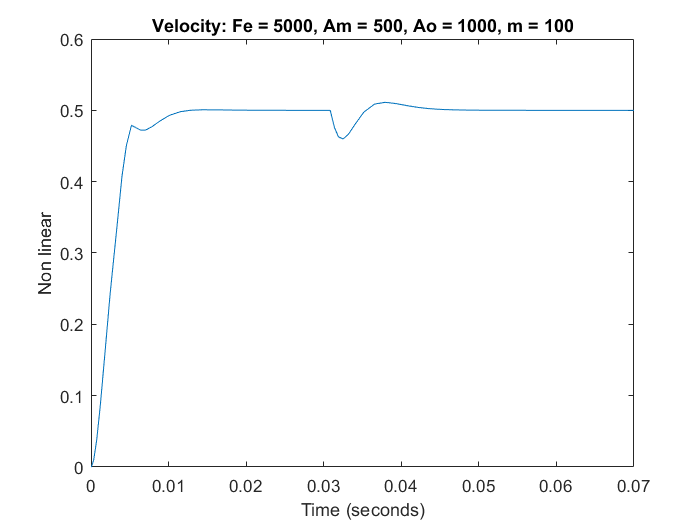
\includegraphics[width=\linewidth]{task3_1_1000.png}
		\caption{Comparison between the two different Ao values}
		\label{fig:task3_1_1000}
	\end{center}
\end{figure}

\subsection{}
Figure \ref{fig:task3_2_1000} shows the step responses for two different values of Ao and now with a mass of 200 kg instead of 100 kg. The system behaves more or less the same as with a mass of 100 kg.
\begin{figure}[H]
	\begin{center}
	
		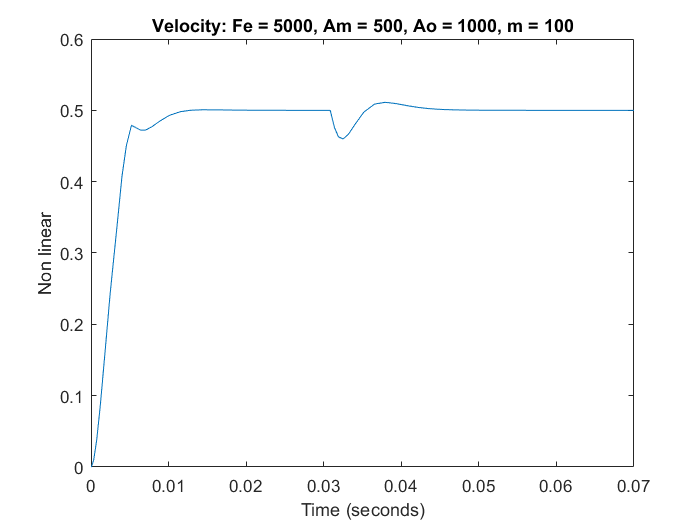
\includegraphics[width=\linewidth]{task3_1_1000.png}
		\caption{Comparison between the two different Ao values}
		\label{fig:task3_2_1000}
	\end{center}
\end{figure}

\subsection{}

Figure \ref{fig:task3_3_1000_freq_1700} shows the step responses for two different values of Ao with a sine wave as noise. The sine wave has a frequency of 1700 rad/s.
\begin{figure}[H]
	\begin{center}
	
		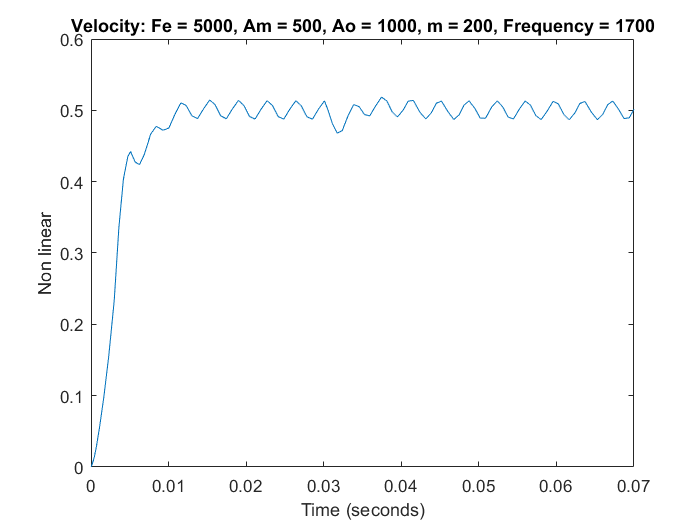
\includegraphics[width=\linewidth]{task3_3_1000_freq_1700.png}
		\caption{Comparison between the two different Ao values}
		\label{fig:task3_3_1000_freq_1700}
	\end{center}
\end{figure}

Figure \ref{fig:task3_3_bode} shows the complementary sensitivity function for the two different Ao values. The magnitude when the frequency is 1700 rad/s is shown which shows that a lower Ao value dampens the noise more. It was hard to find a frequency were the noise dampening were very noticeable but the dampening can be seen in Figure \ref{fig:task3_3_1000_freq_1700} were the noise affects the system less when Ao=1000 compared to Ao=2000.

\begin{figure}[H]
	\begin{center}
	
		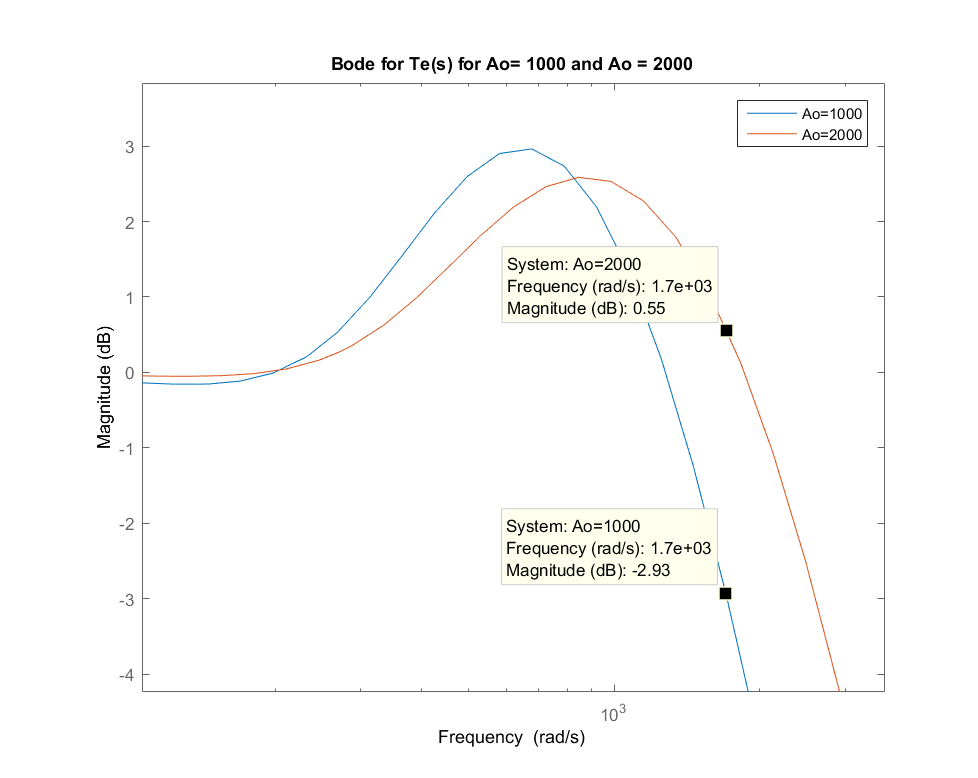
\includegraphics[scale=0.5]{task3_3_bode.png}
		\caption{Comparison between the two different Ao values}
		\label{fig:task3_3_bode}
	\end{center}
\end{figure}


%\end{document}
